\subsection{Unleashing Waves: Exploring Antenna Patterns!}

\begin{tcolorbox}[colback=gray!10, colframe=black, title=E9C03]

What type of radiation pattern is created by two 1/4-wavelength vertical antennas spaced 1/2-wavelength apart and fed in phase?

\begin{enumerate}[label=\Alph*.]
    \item Omni-directional
    \item Cardioid
    \item \textbf{A figure-eight broadside to the axis of the array}
    \item A figure-eight end-fire along the axis of the array
\end{enumerate} \end{tcolorbox}


\subsubsection{Conceptual Background}

To answer this question, we need to explore the following concepts:
\begin{itemize}
    \item The behavior of phased antenna arrays and their radiation patterns.
    \item The effects of spacing and feeding phase on the resulting pattern.
    \item Definitions of radiation terms such as "broadside," "end-fire," and "omni-directional."
\end{itemize}

Phased arrays use interference of waves from multiple antennas to shape the radiation pattern. The pattern depends on the relative phase and spacing between the antennas. For this scenario:
\begin{itemize}
    \item The antennas are spaced 1/2-wavelength apart.
    \item They are fed in phase, meaning the signals from both antennas are synchronized.
\end{itemize}
This setup results in a broadside figure-eight radiation pattern, with maxima perpendicular to the axis of the antennas and nulls along the axis.

\subsubsection{Step-by-Step Explanation}

\begin{enumerate}
    \item \textbf{Understanding the Configuration:} 
    The antennas are 1/4-wavelength vertical elements. Spacing of 1/2-wavelength allows constructive and destructive interference depending on the angle of observation.

    \item \textbf{Interference Analysis:}
    Constructive interference occurs broadside to the array's axis, where signals add up in phase. Destructive interference happens along the axis, where signals cancel each other.

    \item \textbf{Reasoning the Correct Answer:}
    The figure-eight pattern arises broadside to the array because the in-phase feeding ensures maximum reinforcement perpendicular to the antenna axis.

    \item \textbf{Explaining Incorrect Options:}
    \begin{itemize}
        \item \textbf{Option A (Omni-directional):} Incorrect as the pattern is not uniform in all directions due to interference.
        \item \textbf{Option B (Cardioid):} Incorrect because a cardioid pattern requires asymmetry, such as unequal amplitude or phase differences.
        \item \textbf{Option D (Figure-eight end-fire):} Incorrect because an end-fire pattern would require a phase difference designed to favor along-axis radiation.
    \end{itemize}
\end{enumerate}

\subsubsection{Calculation (If Applicable)}

The array factor for two isotropic sources spaced \( d = \lambda/2 \) and fed in phase is:
\[
AF = 2 \cos \left( \frac{\pi d}{\lambda} \cos \theta \right)
\]
Substituting \( d = \lambda/2 \):
\[
AF = 2 \cos \left( \frac{\pi}{2} \cos \theta \right)
\]
This results in maximum radiation at broadside (\( \theta = 90^\circ, 270^\circ \)) and nulls at end-fire (\( \theta = 0^\circ, 180^\circ \)).

\subsubsection{Diagram for Better Understanding}

\begin{figure}
\centering
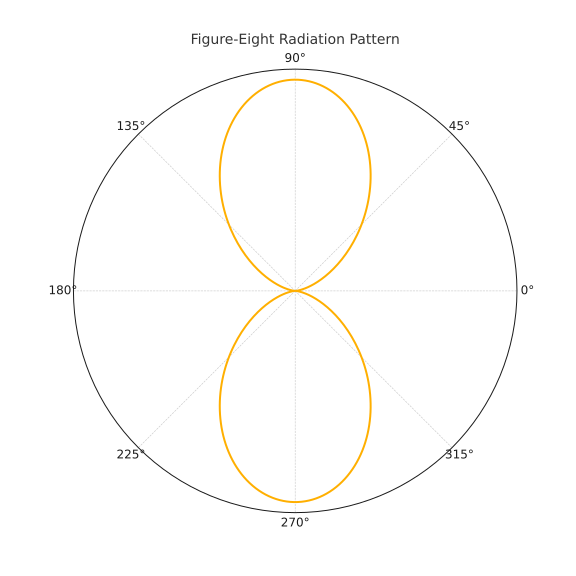
\includegraphics[width=0.3\textwidth]{questions/E9C/figure_eight_pattern.pdf}
\caption{Figure-eight radiation pattern of two 1/4-wavelength vertical antennas spaced 1/2-wavelength apart, fed in phase. The pattern shows maxima broadside to the array's axis and nulls along the axis.}
\end{figure}
% Diagram prompt: Generate an SVG of a figure-eight radiation pattern broadside to the axis of two vertical antennas spaced 1/2-wavelength apart, with nulls along the antenna axis and maxima perpendicular to it.
